\chapter{Fracture}

A critical degradation mechanism observed during the operating lifetime of solid-oxide fuel cell is the formation and propagation of microcracks throughout the functional layer of the anode. These microcracks not only reduce the mechanical integrity of the cell, they are detrimental to its electrochemical performance. They disrupt the ionic transport of fuels within the solid structure, cause delamination around regions with potentially high reaction rates, and result in macroscopic fragmentation of otherwise contiguous cell structures.

The fracture observed in the anode structure is caused by oxidation reactions which occur non-uniformly through the composite structure. Oxygen ions diffuse across the electrolyte to the anode where it reacts with a fuel (typically hydrogen). However, when there is excess oxygen in the anode, it will oxidize the nickel to form nickel-oxide. The phase transformation from nickel to nickel-oxide results in a large volumetric expansion. Due to the heterogeneity of the anode structure, this non-uniform expansion creates considerable internal stresses within the system, especially on the ceramic electrolyte material, which is conventionally chosen to be Yttria-stabalized Zirconia (YSZ). Once enough oxidation has taken place, the transformation strain within the ceramic is relieved by brittle fracture.   

In this chapter, a diffuse-interface model is introduced to study the degradation caused by nickel oxidation within the anode structure of SOFCs and the resulting fracture of the ceramic electrolyte. A particular emphasis is given to the role of the anode microstructure and surface energetics and how these materials design parameters affect critical aspects of the problem such as stress concentration, crack deflection/blunting, and damage accumulation. 

\todo{
Polycrystalline nature of YSZ and the effect of grain boundaries on observed fracture structures
}\\
\todo{
Homogenization Scheme
}\\
\todo{
assumptions
}\\
\todo{
Brittle fracture / unstable fracture
}\\
\todo{
Assymmetrically notched beam
}
\todo{
"quasistatic fracture in a macroscopically isotropic elastic medium with neglible inertial effects" Hakim \& Karma 2005}
\todo{
the phase field representation of the fracture field is essentially a gradient-type or gradient enhanced damage model.}
\section{Background}

\section{The Model}

A first step in developing a model used to study the formation and propagation of cracks is deciding how to represent the crack structure. As with most problems involving sharp interfaces, this is made difficult by the discontinuities of material properties and differences in governing equations across the interface. In the context of brittle fracture, the elastic moduli vary from finite values in the bulk material to zero within the crack and the damaged material can no longer support stresses. The length scale over which this variation occurs is generally considered very small compared and is treated as a boundary within traditional engineering models. However, this treatment requires an explicit representation of the crack surface (usually a mesh) that is rather difficult to carry out in practice. 

As an alternative to traditional methods, the phase field method represents the crack structure implicitly using a scalar field. This allows for the computational convenience of regular grid, finite differencing, and automatic treatment of branching/merging events. However, the ease of implementation comes at a price. An implicit representation of the crack requires that it have a diffuse interface so that the crack field varies continuously from the crack to the bulk material. While the width of the diffuse interface can, in theory, be made very thin, it must be fully resolved for accuracy. This creates a strict trade-off between accuracy and computational viability. In practice, this computational convenience of the diffuse interface typically results in diminished accuracy.  

Several models of brittle fracture employing the phase field framework have been introduced in the literature. The work of Kevin, Kesseler, and Levine (KKL) provides the basic phase field approach to crack formation and propagation used in this thesis. Variations of the KKL model have been successfully applied to structurally and elastically heterogenous systems such as biological composites~\cite{Murali2011} and reinforced composite with misfit strains~\cite{Biner2009} . This work is extended to accommodate the necessary features for application to SOFCs, such as heterogeneous composite structures and internal transformation strains.  

\subsection{Diffuse Interface Formalism}
 
To represent the crack, a scalar field, $\phi$, is introduced and is referred to as the fracture field. Its spatio-temporal evolution designates the regions of material capable of supporting a load from those that have been damaged. It takes a value of $1$ in the undamaged material, a value of $0$ with the crack and pore space, and varies continuously across the crack or pore interfaces. The total free energy of the system can be postulated in terms of the fracture field and is given in Eq.~\ref{eq:free_energy}.

\begin{align}\label{eq:free_energy}
F = \int \left[ \frac{W_{\phi}}{2}|\nabla\phi|^2 + A_{\phi}V(\phi) + E_\phi(\eps)\right]dr	
\end{align}

The first two terms in the integrand of the free energy (Eq.~\ref{eq:free_energy}) are the standard gradient energy and double well terms. The parameters $W_{\phi}$ and $A_{\phi}$ together set the width and energy of the interface of the fracture field. The third term accounts for the strain energy present in the system. The modulating function $g(\phi) = (4-3\phi)\phi^3$ is chosen such that $g(0)=0$ and $g(1)=1$. The result effect is that regions with an elastic strain energy density, $E$, that exceeds the critical threshold value, $E_c$, will tend to form cracks $(\phi=0, g(\phi)=0)$ in order to reduce the total energy. This approach has been shown to accurately reproduce Griffith's criterion and crack branching.

%%%%%%%%%%%%%%%%%%%%%%%%%%%%%%%%%%%%%%%%%%%%%%%%%%%%%%%%%%%%%%%%%%%%%
\subsection{Tension-Compression Split} \label{sec:elastic_split}
%%%%%%%%%%%%%%%%%%%%%%%%%%%%%%%%%%%%%%%%%%%%%%%%%%%%%%%%%%%%%%%%%%%%%

The free energy shown in Eq.~\ref{eq:free_energy} is similar in form to the fracture model proposed by Karma, Kesseler, and Levine (KKL) \cite{Karma2001}\cite{Henry2004}. However, the KKL model has only been formulated and tested for systems under tensile strains. Their approach can not physically model more complex loading situations where the strain may be primarily compressive. In those cases, the KKL model completely ignores all stresses within cracked regions, even though it is reasonable to believe that the crack should transmit compressive stresses. In this section, I propose a modification to the KKL model in order to allow transmission of compressive stresses across the crack faces.

The ability of a crack to transmit compressive or shear stresses is often referred to as a "contact condition." A technique commonly used to represent a contact condition is to split the linear elastic strain energy density into positive and negative parts. In effect, the positive part ($E^+$) contains the energy due to tensile loads while the negative part ($E^-$) contains the energy due to compressive loads. The precise method in which the elastic energy is partitioned is somewhat discretionary and several approaches can be found in the literature \cite{Lancioni2009} \cite{Amor2009} \cite{Miehe2010}. In this study, we take motivation from the work of Amor, Marigo, and Maurini \cite{Amor2009} where the strain is split into spherical and deviatoric parts, $\epsilon = \epsilon_S + \epsilon_D$, and used to reformulate the elastic energy.

\begin{align}\label{eq:energy_split}
E &= \frac{1}{2}\lambda \tr(\eps^e)2 + \mu \tr(\eps^e\cdot\eps^e)\\
E &= \frac{1}{2}K\tr(\eps^e)^2 + \mu\tr(\eps_D^e\cdot\eps_D^e)\\
E &= \frac{1}{2}K\tr^-(\eps^e)^2 + \left[ \frac{1}{2}K\tr^+(\eps^e)^2 + \mu\tr(\eps_D^e\cdot\eps_D^e)\right]\\
E &= E^- + E^+
\end{align}

In undamaged regions, where $\phi=1$, the elastic energy is formed by both positive and negative parts. However, in the region of a fully-formed crack ($\phi = 0$) the energy resulting from tensile loads should be fully relieved while compressive stresses must remain. To achieve this, the partitioned elastic energy is modulated by the crack order parameter as $E = E^- + [g(\phi)+k_l]E^+$. As a crack forms, $\phi\rightarrow 0$ and $g(\phi)\rightarrow 0$ removes the tensile load while leaving the compressive part in tact. The small parameter $k_l$ is referred to as the "residual stress" and is recommended for numerical stability \cite{Amor2009}. The final form of the free energy with an elastic energy partitioned to allow transmission of compresive stresses across the crack face is shown in Eq.~\ref{eq:free_energy_final}.

\begin{align}\label{eq:free_energy_final}
	F &= \int \left[ \frac{W_{\phi}}{2}|\nabla\phi|^2 + A_{\phi}V(\phi) + [g(\phi)+k_l]E^+ + E^-\right]dr\\
	E^+ &= \frac{K}{2} \tr^+(\eps^e)^2 + \mu\tr(\eps_D^e\cdot\eps_D^e)\\
	E^- &= \frac{K}{2} \tr^-(\eps^e)^2
\end{align}

%%%%%%%%%%%%%%%%%%%%%%%%%%%%%%%%%%%%%%%%%%%%%%%%%%%%%%%%%%%%%%%%%%%%%
\subsection{Tension-Compression Asymmetry}
%%%%%%%%%%%%%%%%%%%%%%%%%%%%%%%%%%%%%%%%%%%%%%%%%%%%%%%%%%%%%%%%%%%%%

Typically, a material that fails by brittle fracture is significantly more resistant to fracture under compression than under tension. To account for this, Henry and Levine \cite{Henry2004} introduce a symmetry breaking term into the phase field fracture model. A similar approach is taken in this work, but the term is adapted to satisfy the energy partition discussed previously in Sec.~\ref{sec:elastic_split}. The final form of the linear elastic energy density is given in Eq.~\ref{eq:modified_strain_energy_density} where the symmetry breaking term is $\tfrac{1}{2}(a-1)K\tr^-(\eps^e)^2$. The idea is that when the material is under compression, $\tr^-(\eps^e)$ will be positive and the symmetry breaking term will reduce the elastic energy, assuming $(a>1)$. This modified form prevents the material from cracking under compression.

\begin{align}\label{eq:modified_strain_energy_density}
	E_{\phi} = \frac{K}{2}\tr^-(\eps^e)^2 + [g(\phi)+k_l] \left[K\tr^(\eps)^2 + \mu\tr(\eps_D^e\cdot\eps_D^e) - \frac{a-1}{2}K\tr^-(\eps^e)^2\right]
\end{align}

The constant, $a$, sets the strength of the asymmetry. For $a=1$, there is no asymmetry between tensile and compressive loads, and the elastic energy will take its standard value for an isotropic material. For $a\ge \tfrac{3}{2}$, it is impossible for a crack to form in a region under pure compression. Contours of the modified elastic energy density are plotted in Fig.~\ref{fig:elastic_asymmetry} for the case of biaxial strain. The red line displays the axis of symmetry $\tr(\eps^e)=0$ in the case that $a=1$. For an asymmetry $a\ge \tfrac{3}{2}$ a compressive strain in one direction will still result in a finite elastic energy if there is a large tensile strain in the other principal direction. As a side note, the $(a-1)$ is formulated so that the value of $a$ corresponds with the convention set by Henry and Levine \cite{Henry2004}. The value of $a$ will, in theory, be set by the fracture toughness of the material under tensile versus compression. In practice, however, such a parameterization is difficult to perform and the value of $a$ is chosen from an informed judgement. 

\begin{figure}[h!]
	\begin{center}
	\begin{tabular}{ccc}
		\includegraphics[width=0.3\columnwidth]{ch-fracture/asymmetric_energy/plot_0} &
		\includegraphics[width=0.3\columnwidth]{ch-fracture/asymmetric_energy/plot_15} &
		\includegraphics[width=0.3\columnwidth]{ch-fracture/asymmetric_energy/plot_3}  \\
		(a) & (b) & (c)
	\end{tabular}
	\caption{Contours of $E_{\phi}$ with $a=\{0,\tfrac{3}{2},3\}$ are shown in subfigures (a),(b), and (c), respectively. The red, diagonal line indicates the values of strain where $\tr(\eps^e)=0$. Values of $a>1$ break the symmetry between tensile and compressive stresses so that material under local compression is more resistant to fracture.}
	\label{fig:elastic_asymmetry}
	\end{center}
\end{figure}


%%%%%%%%%%%%%%%%%%%%%%%%%%%%%%%%%%%%%%%%%%%%%%%%%%%%%%%%%%%%%%%%%%%%
\subsection{Order Parameter Evolution}
%%%%%%%%%%%%%%%%%%%%%%%%%%%%%%%%%%%%%%%%%%%%%%%%%%%%%%%%%%%%%%%%%%%%%

In a system undergoing transformation strains, the linear elastic strain energy density, $E$, is given by the elastic strain, $\eps^e$, and determines when the crack becomes energetically favorable. It is expressed generally in Eq.~\ref{eq:elastic_strain_energy_density} using the compliance tensor, $C_{ijkl}$ which contains the elastic moduli. For an isotropic material, the compliance tensor simplifies to $C_{ijkl}=\mu(\delta_{ik}\delta_{jl} + \delta_{il}\delta_{jk}) + \lambda \delta_{ij}\delta_{kl}$, where $\delta$ is the kronecker-delta function defined in Eq.~\ref{eq:kronecker_delta}, and subscripts denote tensor notation. The shear modulus and Lam\'e's first constant are indicated by $\mu$ and $\lambda$, respectively.  The strain energy density is expressed in Eq.~\ref{eq:isotropic_strain_energy_density} for an isotropic material and general eigenstrain. For an isotropic and hydrostatic eigenstrain, the strain energy reduces further to Eq.~\ref{eq:hydrostatic_strain_energy_density}. The bulk modulus depends on the dimensionality, $d$, of the system, $K_d = \lambda+2\mu/d$.


\begin{align}
    E &= \frac{1}{2} C_{ijkl} \epsilon^e_{ij}\epsilon^e_{kl}	 \label{eq:elastic_strain_energy_density}\\
	&= \frac{1}{2} C_{ijkl}\eps_{ij}\eps_{kl} - \frac{1}{2} C_{ijkl}(\eps_{ij}\eps^*_{kl} + \eps_{kl}\eps^*_{ij}) + \frac{1}{2} C_{ijkl}\eps^*_{ij}\eps^*_{kl} \notag\\
	&=\left[\frac{\lambda}{2} \tr(\eps)^2 + \mu \tr(\eps^2)\right]- \left[ \lambda \tr(\eps)\tr(\eps^*) + 2\mu\tr(\eps\,\eps^*) \right] + \left[\frac{\lambda}{2} \tr(\eps^*)^2 + \mu \tr(\eps^*\eps^*)\right]\label{eq:isotropic_strain_energy_density}\\
	&= 	\frac{1}{2} \lambda \tr(\eps)^2 + \mu\tr(\eps^2) - K_d \tr(\eps^*)\tr(\eps) + \frac{1}{2}K_d \tr(\eps^*)^2\label{eq:hydrostatic_strain_energy_density}
\end{align}

\begin{align} \label{eq:kronecker_delta}
	\delta_{ij} =
	\begin{cases}
		1, & i=j\\
		0, & i\ne j
	\end{cases}
\end{align}




%%%%%%%%%%%%%%%%%%%%%%%%%%%%%%%%%%%%%%%%%%%%%%%%%%%%%%%%%%%%%%%%%%%%
\subsection{Order Parameter Evolution New}
%%%%%%%%%%%%%%%%%%%%%%%%%%%%%%%%%%%%%%%%%%%%%%%%%%%%%%%%%%%%%%%%%%%%

Evolution of the fracture order parameter, $\phi$, requires calculation of the stresses $\sigma_{ij}$, strains $\eps_{ij}$, and displacements $u_i$.
The timescale in which the elastic fields relax and the characteristic velocity of crack propagation will determine the quasistatic or dynamic nature of fracture. In this work, we take a quasistatic approach to fracture evolution, which assumes that the timescale on which the elastic field relax is very fast compared to crack propagation. Therefore, a mechanical equilibrium is established throughout the evolution of the fracture field.

To achieve mechanical equilibrium, the displacement fields are initialized and iteratively relaxed until the system reaches the condition for mechanical equilibrium, $\sigma_{ij,j} = 0$. This is done by first calculating the strains from the displacements, $\eps_{ij}=\tfrac{1}{2}(u_{i,j} + u_{j,i})$. The the stress are calculated from the strains and the elastic energy as shown in Eq.~\ref{eq:stress}.


\begin{align*}\label{eq:stress}
	\sigma_{ij} = \frac{\partial E}{\partial \eps_{ij}} 
	=	K\tr^-(\eps^e)\delta_{ij} + (g(\phi)+k_l)\left[ K\tr^+(\eps^e)\delta_{ij} + 2\mu (\eps_D^e)_{ij}\right]
\end{align*}


The displacements can be iteratively relaxed to mechanical equilibrium according to a damped wave equation as shown in Eq.() with the free energy decent determined by the force balance. The time, $t$, is 'fictitious' in the sense that the displacements are assumed to relax instantaneously with respect to the fracture evolution, and it is only used as a dummy variable for the iterative relaxation. The dampening parameter, $\eta$, allows elastic energy to dissipate in transit to a relaxed state while the parameter $\xi$ penalizes high frequencies wavelength and is recomended for using finite differences on collocated grids.  


\begin{align}
\frac{\partial^2 u_i}{\partial t} + (\eta - \xi\nabla^2)\frac{\partial u_i}{\partial t} = -\Gamma \frac{\delta F}{\delta u_i} = \Gamma \frac{\partial \sigma_{ij}}{\partial x_j}
\end{align}



%%%%%%%%%%%%%%%%%%%%%%%%%%%%%%%%%%%%%%%%%%%%%%%%%%%%%%%%%%%%%%%%%%%%%
\section{Validation}
%%%%%%%%%%%%%%%%%%%%%%%%%%%%%%%%%%%%%%%%%%%%%%%%%%%%%%%%%%%%%%%%%%%%%

%%%%%%%%%%%%%%%%%%%%%%%%%%%%%%%%%%%%%%%%%%%%%%%%%%%%%%%%%%%%%%%%%%%%%
\subsection{Eshelby's Inclusion Problem}
%%%%%%%%%%%%%%%%%%%%%%%%%%%%%%%%%%%%%%%%%%%%%%%%%%%%%%%%%%%%%%%%%%%%%

Eshelby's inclusion problem is used to test that the model and implementation properly resolve the elastic fields resulting from an applied transformation strain. This is a classic problem in micro-mechanics that involves an isolated inclusion embedded within an infinite matrix material. An eigenstrain develops within the constrained inclusion due to phase transformation or thermal expansion and causes stress fields throughout the system. J. D. Eshelby solved for the elastic fields in the interior and exterior of an ellipsoidal inclusion for a given eigenstrain \cite{Eshelby1957, Eshelby1959} . In this section, the results of simulation are compared to his analytical predictions. 



\begin{figure}[h!]
	\begin{center}
	\includegraphics[width=0.6\columnwidth]{ch-fracture/eshelby/inclusion}	
	\caption{The eigenstrain is set to $\eps_T=0.01$ within a spherical inclusion (orange). Contours of the elastic field exterior to the inclusion are plotted within a two-dimensional slice for one component of the stress, $\sigma_{xx}$.}
	\label{fig:eshelby_3d}
	\end{center}
\end{figure}

A test system is configured with a spherical inclusion of radius $a=15$ embedded within the matrix material. Due to the finite limitations of computational simulation, the matrix material will be constrained to a spherical domain that is a factor of six larger in linear size than the inclusion. The system is first coarsened with conserved dynamics to establish a diffuse interface. The materials are set to be elastically homogeneous with Lame's constant and shear modulus given by $\lambda = 150$ and $\mu = 75$ GPa, resulting in $\nu = 1/3$. An eigenstrain, $\eps_T=0.01$, is applied only within the inclusion, and elastic fields are established throughout the system due to this structural inhomogeneity. Figure~\ref{fig:eshelby_3d} shows a three dimensional rendering of the system with a two dimensional slice cutting through the matrix. Contours of one component of the stress tensor, $\sigma_{xx}$, are plotted along the slice and indicate areas of tensile and compressive stress with variations in red and blue color.  

\begin{figure}[h!]
	\begin{center}
	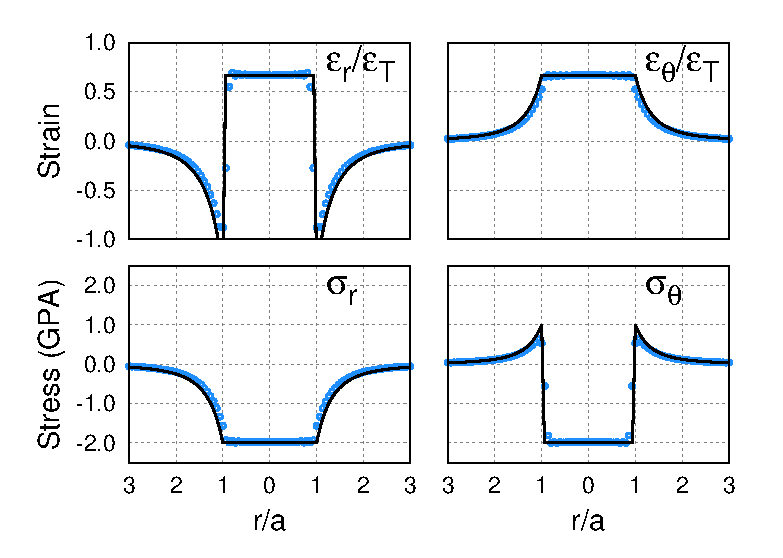
\includegraphics{ch-fracture/eshelby/stress_strain}
	\caption{The subplots display values of the radial and tangential components of the stress and strain against the radial distance from the inclusion's center. The strains are normalized by the eigenstrain in the inclusion, $\eps_T=0.01$. The simulation results (blue symbols) agree closely with analytical predictions (solid black line).}  
	\label{fig:eshelby_results}
	\end{center}
\end{figure}


Insight into the elastic fields that develop as a result of the eigenstrain can be gained through a series of cutting and welding operations envisioned by Eshelby~\cite{Eshelby1957}. If one were to remove the inclusion from the matrix, it would undergo a stress-free strain equal to the eigenstrain. Now, apply a stress that forces the inclusion to its original size and return it to the matrix. An expansion would be observed in the inclusion, but less than that of the eigenstrain. Meanwhile, the matrix would feel compressive strains in the radial direction and tensile strains in the direction tangential to the inclusion surface. Eschelby found that the strain is constant within the inclusion and falls off with the cube of the radial distance within the matrix material. The solutions are summarized in Eq.~\ref{eq:eshelby} \cite{Mura1982}.

\begin{equation}
\begin{alignedat}{2}
	\label{eq:eshelby}
		\eps_r &= \eps_t = \frac{1}{3}\frac{1+\nu}{1-\nu} \eps_T, &&\qquad r<a \\
		\eps_r &= -2\eps_t= \frac{-2}{3} \frac{1+\nu}{1-\nu} \left(\frac{a}{r}\right)^3 \eps_T, &&\qquad r>a
\end{alignedat}
\end{equation}


Figure~\ref{fig:eshelby_results} compares simulation results to the analytical predictions along a line that extends radially from the center of the inclusion and into the matrix. The radial distance is normalize by the inclusion radius, $a=15$ and the strains are normalized by the isotropic eigenstrain within the inclusion, $\eps_T = 0.15$. The data values, shown as blue symbols, agree closely to the analytical predictions, which are plotted as solid black lines. Notice that the strains within the inclusion $r/a<1$ are constant and about 70\% of the applied eigenstrain.

\subsection{Three-Point Bending Test}
 
\section{Results}
\section{Discussion}